\chapter{Experiment}
\label{ch:experiment}

In the Experiment an optical transmitter was simulated in OptSim. The Experiment was divided in three sub-projects.

\section{Project 1}
\label{sec:P1}
For the Experiment an OptiSim Example of a 50~\% RZ-OOK-Transmitter was used. Figure \ref{fig:P1_aufbau} shows this example\footnotemark[3]. In the upper left-hand side theres the PRBS which generates a pseudo-random bit-stream. A logical connection path (green) leads to eh


\begin{figure}%
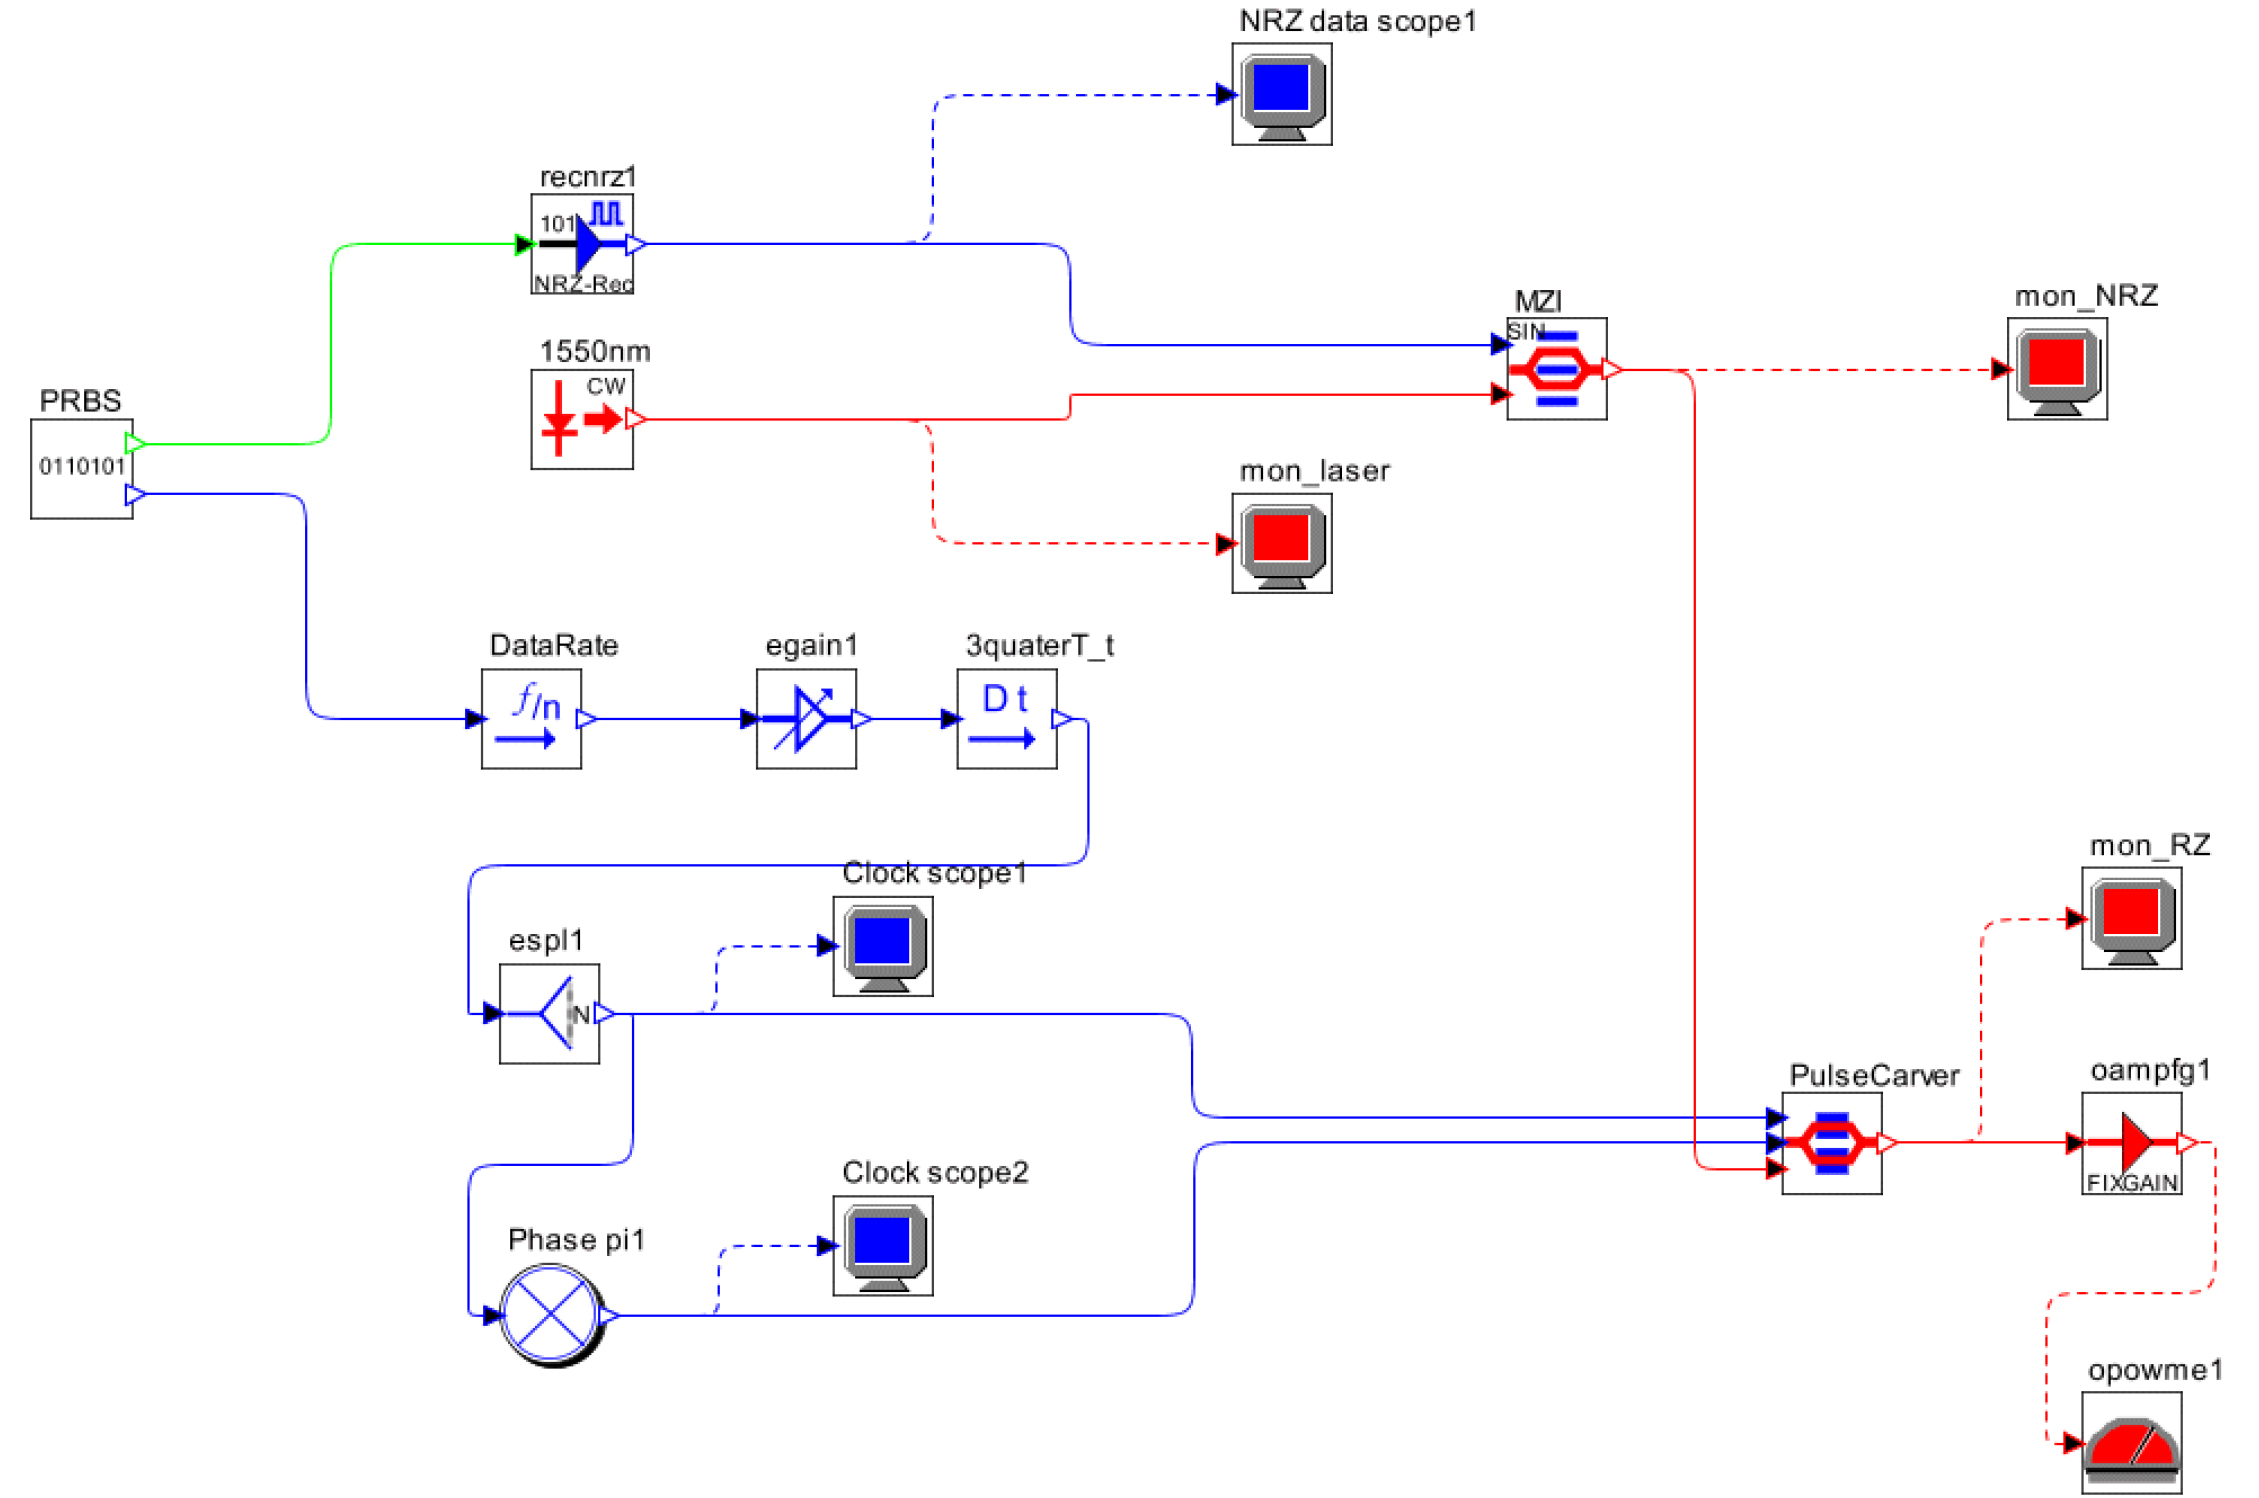
\includegraphics[width=\columnwidth]{Grafiken/P1_aufbau.jpg}%
\caption{OptiSim Sample-Mode example of a 50~\% RZ-OOK-Transmitter}%
\label{fig:P1_aufbau}%
\end{figure}


\footnote[3]{Materials for the Preparation of Experiment 7: Simulation of Optical Transmitters}
